\documentclass{article}
\usepackage[margin=0.5in]{geometry}
\usepackage{graphicx, xcolor, colortbl, array, booktabs, tikz, enumitem, multicol, setspace}
\usepackage[hidelinks]{hyperref}
\usepackage{titlesec}
\usepackage{pagecolor}
\pagestyle{empty}

% Define custom colors
\definecolor{pspblue}{HTML}{1C6B6B}
\definecolor{tsrgreen}{HTML}{19796B}
\definecolor{graytext}{gray}{0.4}
\definecolor{lightgray}{gray}{0.9}
\definecolor{midgray}{gray}{0.7}
\definecolor{chartgreen}{HTML}{6BCABA}
\definecolor{chartgray}{HTML}{D5D5D5}

\titleformat{\section}{\Large\bfseries\color{pspblue}}{}{0em}{}
\titleformat{\subsection}{\bfseries\color{pspblue}}{}{0em}{}

\begin{document}
\pagecolor{pspblue!15}
\section*{Performance Share Plan (PSP) \textnormal{(audited)}}

\subsection*{Targets}
The 2022 PSP award is measured against PBT growth and relative total shareholder returns (TSR) over a three-year period between FY 2021 to FY 2024. Any shares that vest under the PSP award are subject to a two-year post-vest holding period for serving Executive Directors.

\noindent\begin{minipage}[t]{0.45\textwidth}

\textbf{PBT growth measure}
\par\vspace{1em}\par % space between heading and table in order to align both tables side by side
\begin{tabular}{
>{\raggedright}b{0.3\textwidth} 
>{\raggedright}b{0.3\textwidth} 
>{\raggedleft\arraybackslash}b{0.3\textwidth}}

\textbf{Performance level} & \textbf{Growth in PBT} & \textbf{\% of PBT tranche that will vest} \\
\arrayrulecolor{pspblue}\hline\arrayrulecolor{black}
Below threshold & Below 5\% p.a. & 0\% \\
Threshold & 5\% p.a. & 15\% \\
Exceptional & 12\% p.a. or above & 100\% \\
\bottomrule
\end{tabular}
\end{minipage}
\hfill
\begin{minipage}[t]{0.45\textwidth}
\textbf{Relative TSR measure}
\par\vspace{1.15em}\par % space between heading and table in order to align both tables side by side
\begin{tabular}{
>{\raggedright}b{0.3\textwidth} 
>{\raggedright}b{0.3\textwidth} 
>{\raggedleft\arraybackslash}b{0.3\textwidth}}
\textbf{Performance level} & \textbf{TSR ranking vs comparators} & \textbf{\% of TSR tranche that will vest} \\
\arrayrulecolor{pspblue}\hline\arrayrulecolor{black}
Below threshold & Below median & 0\% \\
Threshold & At median & 15\% \\
Exceptional & At or above upper quartile & 100\% \\
\bottomrule
\end{tabular}
\end{minipage}

\subsection*{Outcome}
The 2022 PSP award will vest at \textbf{74.3\%} of maximum, reflecting strong performance on both PBT growth (11.1\% p.a., vesting at 88.9\%) and relative TSR (ranked between median and upper quartile, vesting at 44.6\%). Share price appreciation also contributed to the award values received by Andrew Livingston (\pounds135,214) and Paul Hayes (\pounds72,037).

\vspace{2em}

\noindent
\begin{minipage}{0.48\textwidth}
\centering
\textbf{\textcolor{pspblue}{PBT growth outcome}}\\
\textcolor{graytext}{\small Worth 67\% of maximum opportunity under award}

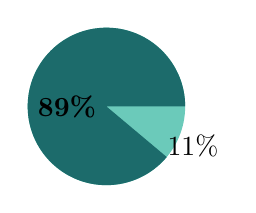
\begin{tikzpicture}
\draw[fill=chartgreen, draw=none] (0,0) circle (1);
\draw[fill=pspblue, draw=none] (0,0) -- (0:1) arc (0:320:1) -- cycle;
\node at (-0.5,0) {\textbf{89\%}};
\node at (1.1,-0.5) {11\%};
\end{tikzpicture}

\textcolor{pspblue}{\rule{10pt}{10pt}} Actual outcome \hspace{1em}
\textcolor{chartgreen}{\rule{10pt}{10pt}} Target not reached
\end{minipage}
\hfill
\begin{minipage}{0.48\textwidth}
\centering
\textbf{\textcolor{tsrgreen}{Relative TSR outcome}}\\
\textcolor{graytext}{\small Worth 33\% of maximum opportunity under award}

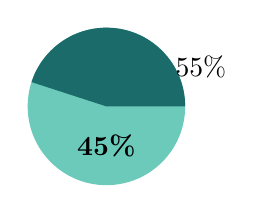
\begin{tikzpicture}
\draw[fill=chartgreen, draw=none] (0,0) circle (1);
\draw[fill=pspblue, draw=none] (0,0) -- (0:1) arc (0:162:1) -- cycle;
\node at (0,-0.5) {\textbf{45\%}};
\node at (1.2,0.5) {55\%};
\end{tikzpicture}

\textcolor{pspblue}{\rule{10pt}{10pt}} Actual outcome \hspace{1em}
\textcolor{chartgreen}{\rule{10pt}{10pt}} Target not reached
\end{minipage}

\end{document}
